\section{Finite-Volume Discretization}

The governing equation was discretized using the finite-volume method on a structured Cartesian mesh. In this approach, the computational domain is divided into a collection of non-overlapping control volumes, and the governing equation is enforced over each control volume individually. Unlike finite-difference methods, which approximate the governing equation directly at discrete points, the finite-volume method is derived from the integral form of the conservation law, thereby ensuring local conservation within every control volume.

Expressing the Laplace operator in divergence form and integrating over an arbitrary control volume yields

\begin{equation}
\iint_{CV}\nabla\cdot\left(\nabla T\right)\,dA=0
\label{eq:fvm_integral}
\end{equation}

Applying the divergence theorem converts the volume integral into a surface integral over the control-volume boundary,

\begin{equation}
\oint_{CS}\nabla T\cdot\mathbf{n}\,ds=0
\label{eq:gauss}
\end{equation}

where $\mathbf{n}$ denotes the outward unit normal vector to the control surface. Equation~\ref{eq:gauss} states that, at steady state and in the absence of internal heat generation, the net diffusive heat flux through the boundary of every control volume is zero.

The computational stencil and notation adopted throughout the discretization procedure are illustrated in Figure~\ref{fig:grid}.

\begin{figure}[H]
    \centering
    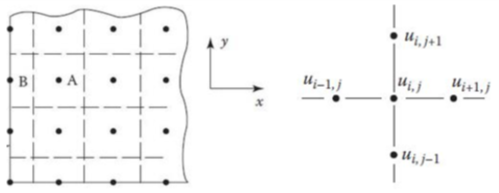
\includegraphics[width=0.60\textwidth]{figures/grid.png}
    \caption{Computational stencil and control-volume notation used in the finite-volume discretization.}
    \label{fig:grid}
\end{figure}

To achieve second-order spatial accuracy, the temperature gradients at the control-volume faces are approximated using central differences. For a uniform Cartesian mesh, the temperature gradient at the east face of a control volume is approximated by

\begin{equation}
\left.\frac{\partial T}{\partial x}\right|_{i+\frac12}
=
\frac{T_{i+1}-T_i}{\Delta x}
+
\mathcal{O}(\Delta x^2)
\label{eq:face_gradient}
\end{equation}

An analogous expression is obtained for the remaining control-volume faces in both coordinate directions.

Substituting the face-gradient approximations into Equation~\ref{eq:gauss} and evaluating the fluxes across the four faces of each control volume yields the discrete form of the governing equation,

\begin{equation}
\frac{T_{i+1,j}-2T_{i,j}+T_{i-1,j}}{\Delta x^2}
+
\frac{T_{i,j+1}-2T_{i,j}+T_{i,j-1}}{\Delta y^2}
=
0
\label{eq:laplace_discrete}
\end{equation}

For the present study, a uniform Cartesian mesh is employed such that

\[
\Delta x=\Delta y.
\]

Under this condition, Equation~\ref{eq:laplace_discrete} provides a second-order accurate approximation of the continuous Laplace equation throughout the computational domain.

The resulting system of algebraic equations is coupled through the neighboring control-volume temperatures and therefore cannot be solved independently for each cell. An iterative solution procedure is consequently required to obtain the numerical temperature distribution.

